\documentclass{ximera}

\usepackage{microtype}
\usepackage{tikz}
\usepackage{tkz-euclide}
\usetkzobj{all}
\tikzstyle geometryDiagrams=[ultra thick,color=blue!50!black]

\renewcommand{\epsilon}{\varepsilon}



\title{Hyperbolic lunes and triangles}

\begin{document}
\begin{abstract}
In this activity, we explore the areas of lunes and triangles in
hyperbolic geometry.
\end{abstract}
\maketitle

We know that the area of a triangle in spherical geometry with angles
$\alpha$, $\beta$, and $\gamma$ is given by
\[
R^2(\alpha+\beta+\gamma - \pi).
\]
\begin{problem}
  Briefly sketch the line of reasoning used to deduce the formula for
  the area of a triangle in spherical geometry.
\end{problem}

We will attempt to use reasoning anagous to the reasoning we used to
deduced the formula above to deduce the formula for a triangle with
angles $\alpha$, $\beta$, and $\gamma$ in hyperbolic geometry.

\section{Hyperbolic lunes}

Consider the following diagram on the Klein disk, central projection
of hyperbolic geometry:
\begin{image}
  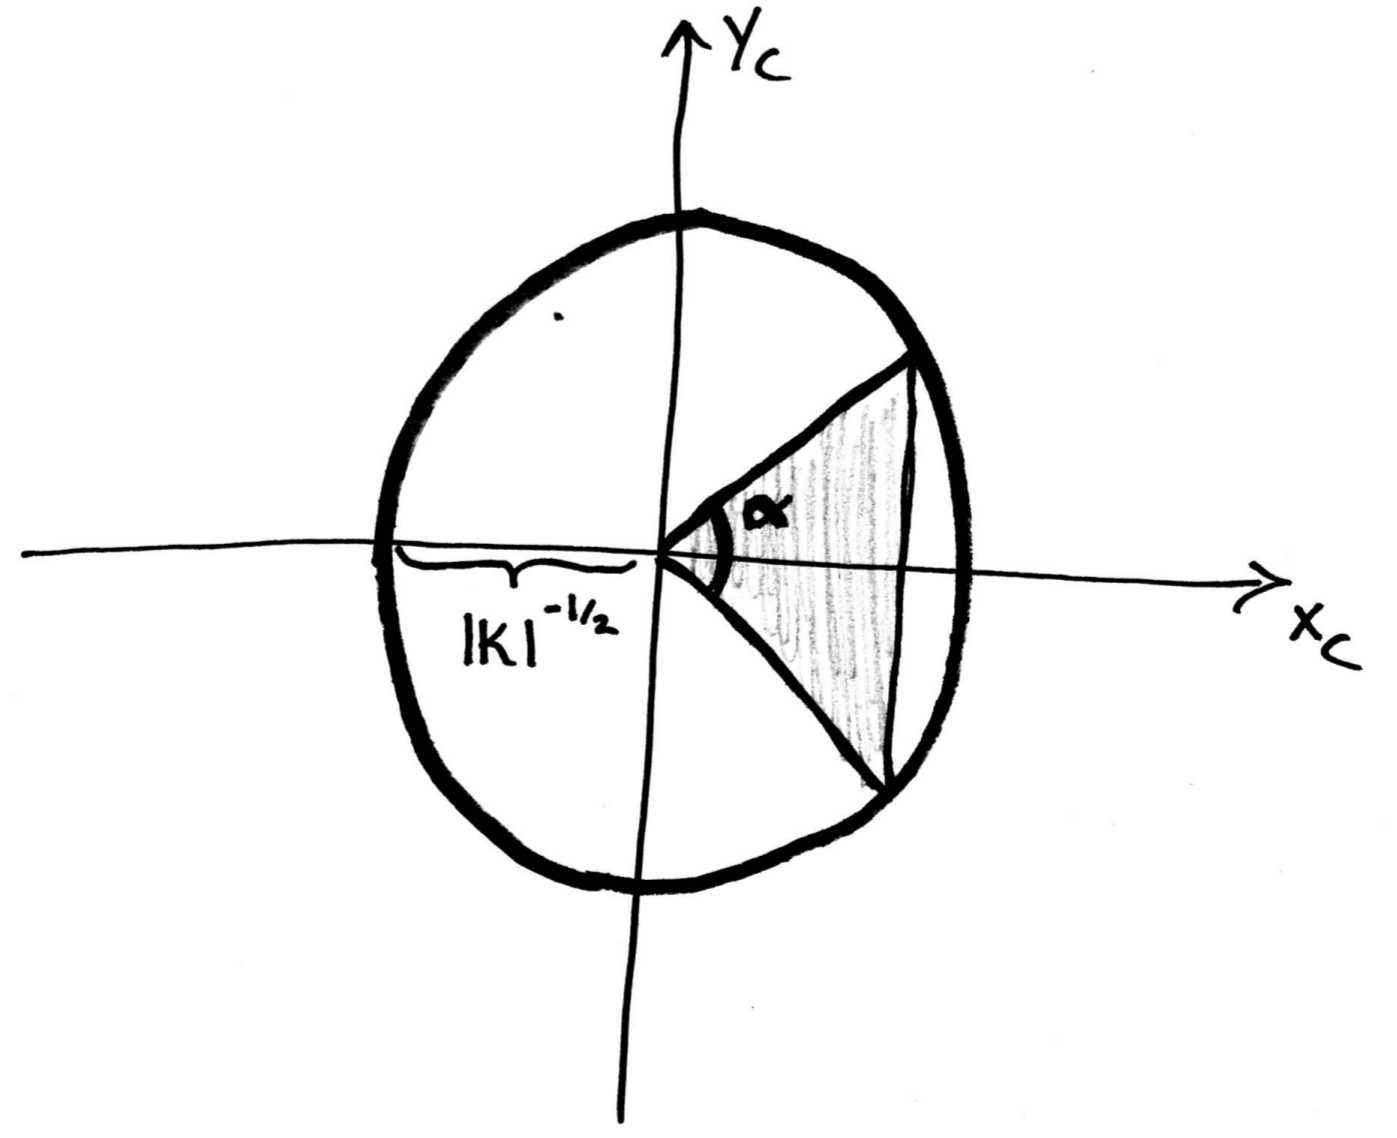
\includegraphics[width=3in]{diagramOfHyperbolicLune.png}
\end{image}

\begin{definition}
  We will define an \dfn{$\boldsymbol\alpha$-lune} in hyperbolic
  geometry to be a triangle with an angle of measure $\alpha$ where
  verticies opposite of $\alpha$ are at infinity.
\end{definition}

We have seen that
\begin{align*}
  \int_{L_c} \sqrt{
  \det
  \begin{bmatrix}
    \dd[X]{x_c}\bullet_K \dd[X]{x_c} & \dd[X]{y_c}\bullet_K \dd[X]{x_c} \\
    \dd[X]{x_c}\bullet_K \dd[X]{y_c} & \dd[X]{y_c}\bullet_K \dd[X]{y_c}
  \end{bmatrix}
  }\d x_c\d y_c &=
  \int_{L_c} \sqrt{\det P_c}\d x_c\d y_c\\
  &=\int_{L_c} \left(K\left(x_c^2+y_c^2\right)+1\right)^{-3/2} \d x_c\d y_c.
\end{align*}


In what follows, we will assume that $K=-1$. This will simplify the
computations somewhat. Once the mathematician is familier with this
case, the general case when $K<0$ will fall easily.


\begin{problem}
  Convert
  \[
  \int_{L_c} \left(-\left(x_c^2+y_c^2\right)+1\right)^{-3/2} \d x_c\d y_c
  \]
  to polar coordinates and compute the integral.
  \begin{hint}
    Redraw the picture above with $\alpha = 2\beta$ and $K=-1$.
  \end{hint}
  \begin{hint}
    Recall that to covert to polar coordinates, set
    \begin{align*}
      r &= \sqrt{x_c^2+y_c^2},\\
      \theta &= \arctan(y_c/x_c),
    \end{align*}
    and replace $\d x_c\d y_c$ with $r\d r\d \theta$.
  \end{hint}
  \begin{hint}
    At some point you may wish to use the following idenities:
    \[
    \begin{split}
      \cos^2\theta + \sin^2\theta &=1\\
      \cos^2\theta &= 1-\sin^2\theta
    \end{split}
    \qquad
    \begin{split}
      \cos^2\beta + \sin^2\beta &=1\\
      \cos^2\beta &= 1-\sin^2\beta
    \end{split}
    \]
    So
    \begin{align*}
      \cos^2\theta - \cos^2\beta &= 1 - \sin^2\theta - \left(1-\sin^2\beta\right)\\
      &= \sin^2\beta - \sin^2\theta.       
    \end{align*}
  \end{hint}
  \begin{hint}
    Finally, it will also be helpful to recall that when $a>0$,
    \[
    \int \frac{1}{\sqrt{a - t^2}} \d t = \arcsin\left(\frac{t}{\sqrt{a}}\right) + C.
    \]
  \end{hint}
  \begin{freeResponse}
    Write
    \[
    \int_{L_c} \left(-\left(x_c^2+y_c^2\right)+1\right)^{-3/2} \d x_c\d y_c
    = \int_{-\beta}^\beta \int_0^{\frac{\cos \beta}{\cos\theta}}\left(-r^2+1\right)^{-3/2} r\d r\d \theta.
    \]
    Integrating this from the inside-out we find
    \begin{align*}
      &= \int_{-\beta}^\beta \eval{\left(-r^2+1\right)^{-1/2}}_0^{\frac{\cos \beta}{\cos\theta}}\d \theta\\
      &= \int_{-\beta}^\beta \left(-\left(\frac{\cos \beta}{\cos\theta}\right)^2+1\right)^{-1/2}\d\theta - \eval{\theta}_{-\beta}^\beta\\
      &= \int_{-\beta}^\beta \left(1-\frac{\cos^2 \beta}{\cos^2\theta}\right)^{-1/2}\d \theta -2\beta\\
      &= \int_{-\beta}^\beta \left(\frac{\cos^2\theta - \cos^2 \beta}{\cos^2\theta}\right)^{-1/2} \d \theta-\alpha\\
      &= \int_{-\beta}^\beta \frac{\cos\theta}{\sqrt{\cos^2\theta - \cos^2 \beta}}\d \theta - \alpha.
    \end{align*}
    Now apply a trigonometric substitution,
    \begin{align*}
      &= \int_{-\beta}^\beta \frac{\cos\theta}{\sqrt{\sin^2\beta - \sin^2 \theta}}\d \theta- \alpha\\
      &= \eval{\arcsin\left(\frac{\sin\theta}{\sin\beta}\right)}_{-\beta}^\beta - \alpha\\
      &= \arcsin\left(\frac{\sin\beta}{\sin\beta}\right)- \arcsin\left(\frac{\sin(-\beta)}{\sin\beta}\right)- \alpha\\
      &= \arcsin(1)-\arcsin(-1)-\alpha\\
      &= \frac{\pi}{2}-\frac{-\pi}{2}-\alpha\\
      &= \pi-\alpha.
    \end{align*}
  \end{freeResponse}
\end{problem}


\section{Hyperbolic triangles}

Now we will use our knowledge of the areas of hyperbolic lunes to
compute the area of an \textit{ideal triangle} in hyperbolic geometry.

\begin{definition}
  An \dfn{ideal triangle} is a triangle in hyperbolic geometry with
  its vertices at infinity.
\end{definition}

We would like to know the area of an ideal triangle.

\begin{problem}
  
\end{problem}

Use the diagram below 


compute area of ideal triangle (use stereographic proj)

Compute area of ideal hexagon

consider the funky drawing
compute the are of a circle hyperbolic geometry.




\end{document}
